\chapter{Anexos}

\section{Código Fuente}

En esta sección se adjunta el código fuente completo del proyecto Blink LED.

\subsection{Archivo main.c}
\lstinputlisting[language=C, caption={Lógica principal en C}]{sources/blink_led/src/main.c}

\subsection{Archivo crt.s}
\lstinputlisting[language=C, caption={Archivo de startup en ensamblador}]{sources/blink_led/src/crt.s}

\subsection{Script del Enlazador (linker.ld)}
\lstinputlisting[language=C, caption={Configuración del enlazador}]{sources/blink_led/src/linker.ld}

\subsection{Makefile}
\lstinputlisting[language=make, caption={Automatización de la compilación}]{sources/blink_led/Makefile}

\newpage

\section{Extractos de documentos}

\subsection{Mapa de memoria}
\label{annex:mapa_memoria}

\begin{figure}[!ht]
    \centering
        \includegraphics[page=34, trim=4cm 4.8cm 2cm 5.45cm, clip=true, height=17cm]{../commons/stm32f103c8.pdf}
    \caption{mapa de memoria del STM32F103x8.}
\end{figure}

